\startchapter{Web Application}
\label{chapter:webSite}
\section{Web Tools}
%%%%%%%%%%%%%%%%%%%%%%%
\subsection{The Classification Tool} \label{sec:toolClassification}
To investigate a trojan, users select attributes via an easy to use User Interface (UI).
Once the attributes are chosen, the tool performs the necessary analysis using matrix $\mathbf{R}$ and displays the resulting directed graph.
Suppose an attacker decides to insert the trojan described in Section~\ref{sec:techniqueClassification}. % and shown in Fig.~\ref{fig:full2}.
The tool provides the directed graph shown in Fig.~\ref{fig:visualRepresentaion} from the selected attributes, which eliminate the
need for manual analysis of the matrix.
Note that Fig.~\ref{fig:visualRepresentaion} is the same as Fig.~\ref{fig:full2} which was constructed by hand.
This verifies the results obtained using the classification tool.
\begin{figure}[h]
	\centering
	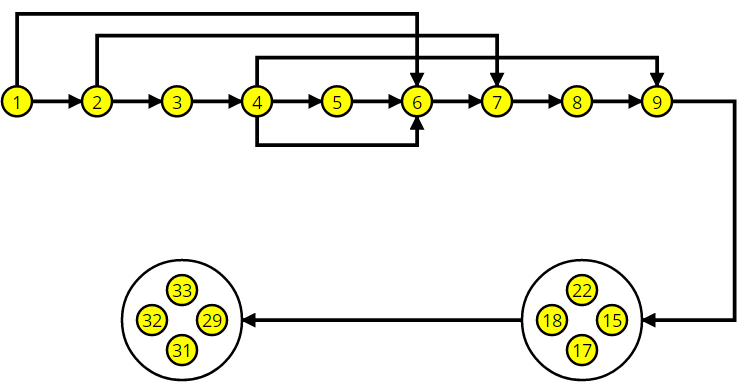
\includegraphics[width=0.9\linewidth]{figures/visualRepresentaion}
	\caption{The directed graph obtained by analyzing a hardware trojan with the classification tool.}
	\label{fig:visualRepresentaion}
\end{figure}
\begin{figure}[h]
	\centering
	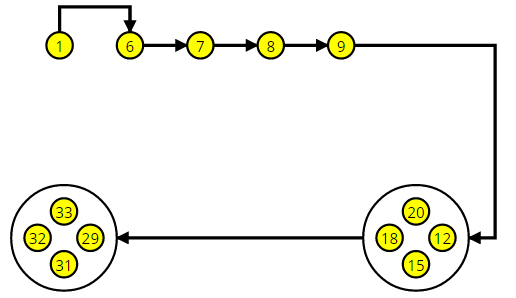
\includegraphics[width=0.75\linewidth]{figures/visualRepresentaion2}
	\caption{The directed graph after attribute $2$ is removed.}
	\label{fig:visualRepresentaion2}
\end{figure}

If the design phase (attribute $2$) takes place in a secure location, an attacker will conclude that
it is not possible to insert the trojan in this phase.
To determine the possible trojans that can be inserted without access to the design phase,
attribute $2$ should be removed from Fig.~\ref{fig:visualRepresentaion}.
The classification tool provides an attribute removal feature.
When an attribute is removed, the directed graph is recreated based on the new matrix $\mathbf{R}$.
The result of removing attribute $2$ is shown in Fig.~\ref{fig:visualRepresentaion2}.
The new graph clearly shows that compromising the design is still possible, but it must be done from the specification phase (attribute $1$).
The possible locations remain the same, but the potential effects of the trojan have changed.
Without access to the design phase (attribute $2$), the trojan cannot be composed of combinational logic (attribute $17$) or be externally triggered (attribute $22$).
Even though the attributes change in functionality (attribute $12$) and always on (attribute $20$) were not selected,
the tool determined that these attributes are possible.

The classification tool automatically generates a severity/coverage vector for use with the evaluation tool described in Section~\ref{sec:toolDetection}.
The identification and severity vectors describing the trojan in Fig.~\ref{fig:visualRepresentaion} are shown in Fig.~\ref{fig:classificationSeverity}.
The trojan classification data is saved in the database along with the identification and severity/coverage vectors.
\begin{figure}
	\centering
	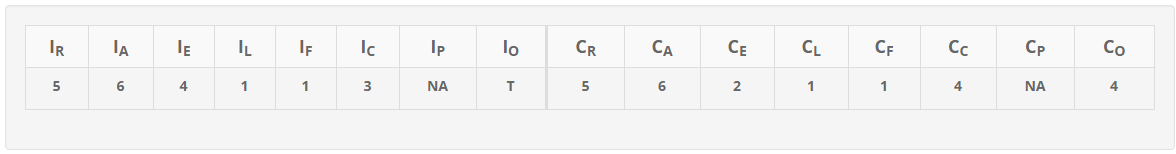
\includegraphics[width=1\linewidth, height = 3cm]{figures/classificationSeverity}
	\caption{The identification and severity vectors generated by the classification tool for the trojan in Fig.~\ref{fig:visualRepresentaion}.}
	\label{fig:classificationSeverity}
\end{figure}

%%%%%%%%%%%%%%%%%%%%%%%
\subsection{The Evaluation Tool} \label{sec:toolDetection}
The HTS provides a series of drop-down lists to create a coverage vector for a new detection method.
This vector is stored in the database along with a description of the method.
The evaluation tool provides a simple means of searching the database for previously saved detection method coverage vectors and trojan severity vectors.
Once a detection method and a trojan have been selected, a user can use the compare button to perform a comparison of the coverage and severity vectors.
For example, the results of a comparison are shown in the bottom row of Fig.~\ref{fig:comparison}.
A $1$ is displayed when the detection method has a value greater than or equal to the corresponding trojan value, and a $0$ otherwise.
The zeros in Fig.~\ref{fig:comparison} indicate that the detection method may fail to detect
the trojan based on the insertion point (\textit{$I_R$}) and the logic type (\textit{$I_F$}).

While the evaluation tool can be employed for individual comparisons, its greatest potential is with a centralized database.
Currently the tool only provides comparisons of trojans and detection methods entered by the user.
Universal adoption of the HTS will provide a centralized database of all known detection methods and trojans.
This database will allow the evaluation tool to provide extensive comparison results.
Attackers can use this information to design trojans and defenders can use it to develop security solutions.
\begin{figure}[]
	\centering
	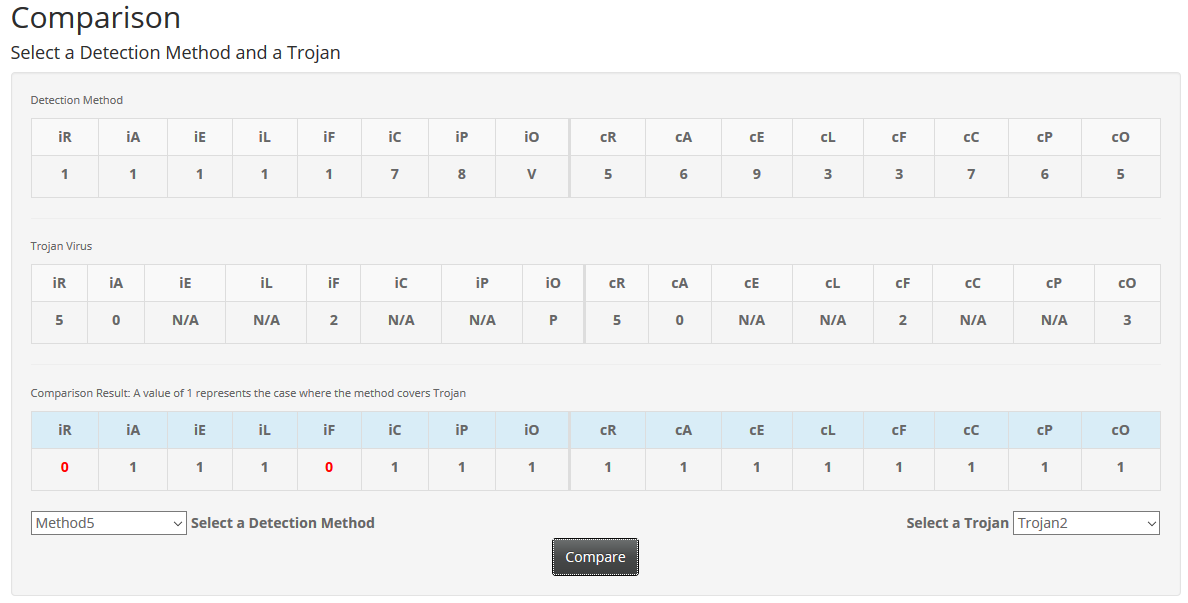
\includegraphics[width=1\linewidth]{figures/comparison}
	\caption{A comparison of coverage and severity vectors.}
	\label{fig:comparison}
\end{figure}